\section{Kodierung von \ttt}
\label{chap:ttt_encoding}

Das \acl{TTT} Spielfeld besteht aus neun Slots, die entweder leer oder durch ein Symbol belegt sind.  
Ein Spielfeld kann daher als Folge von Bits betrachtet werden. 
Diese Form der Kodierung wird als Bitboard bezeichnet und genutzt zur speichereffizienten Beschreibung von Spielfeldern, die mit Bitoperationen manipuliert werden können. \cite[S. 86]{slateCHESSNorthwesternUniversity1983}

Werden die Slots, beginnend bei $0$, von oben links nach unten rechts indexiert, kann der Zustand eines Spielfeldes als neunstellige Binärzahl $B_G$ ausgedrückt werden. 
Der Index eines Slots ist der Exponent zur Basis 2. 
Beispielsweise beschreibt der Zustand $0_2$ ein leeres Spielfeld und $111000000_2$ die Konstellation, in der die Slots $0-5$ frei sind und die letzte Reihe gefüllt ist, wie in \cref{fig:ttt_index_and_bottomrow} dargestellt.

\begin{figure}
    \centering
    \begin{subfigure}[b]{0.45\textwidth}
      \centering
      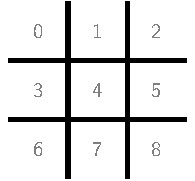
\includegraphics[scale=0.7]{ttt_boards/ttt_index.pdf}
      \caption{Indexierung der Slots}
      \label{fig:ttt_index}
    \end{subfigure}
    \begin{subfigure}[b]{0.45\textwidth}
      \centering
      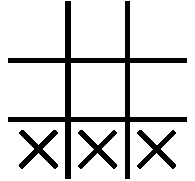
\includegraphics[scale=0.7]{ttt_boards/ttt_bottom_row_x.pdf}
      \caption{Zustand $111000000_2$}
      \label{fig:ttt_bottom_row_x}
    \end{subfigure}
    \caption{\acs{TTT} Indexierung und Beispiel für $B_G$}
    \label{fig:ttt_index_and_bottomrow}
\end{figure}

Jedoch sind neun Bits nicht ausreichend, da zwischen zwei verschiedenen Symbolen und somit insgesamt drei Zuständen pro Slot unterschieden werden muss. 
Daher muss die Konstellation des Spielfeldes für jedes Symbol in einem dedizierten Bitboard kodiert werden, die im Folgenden als $B_X$ und $B_O$ bezeichnet werden.

Durch Konkatenation der beiden Bitboards \bzw Binärzahlen ist die Kodierung des gesamten Spielfeldes mit Unterscheidung der Symbole  für einen Zustand $s$ in einer 18-stelligen Binärzahl möglich. 
Diese wird als $B_{s}$ bezeichnet. 
Dabei wird festgelegt, dass die ersten neun Bits für $B_O$ und die anderen für $B_X$ stehen. Der Wert von $B_s$ zur Basis $10$ kann mit \cref{eq:bitboard_bs} eineindeutig berechnet werden. 


\begin{equation}\label{eq:bitboard_bs}\equationentry{Berechnung des Zustandsidentifikators $B_s$}
   B_s= \sum_{i=9}^{17}2^{i}\cdot \mathbbm{1}_{X_i=true} + \sum_{i=0}^{8}2^{i}\cdot \mathbbm{1}_{O_i=true}
\end{equation}

Durch Logische OR Verknüpfung der Bitboards beider Symbole kann die neunstellige Spielfeldkodierung $B_G$ vom Anfang erreicht werden, die nicht zwischen Symbolen unterscheidet: $B_X \lor B_O = B_G$. 
Die Bits in $B_G$ mit Wert False sind die freien Slots und kodieren die Menge der legalen Aktionen $A$. 
Somit hat ein Agent maximal neun mögliche Aktionen, die im Interval $[0; 8]$ liegen. 
Wird eine Aktion von einem Spieler durchgeführt, so wird der Index des von ihm belegten Slot in seinem eigenen Bitboard auf True gesetzt.
Ein Beispiel für eine Kodierung einer Spielfeldkonstellation ist in \cref{fig:ttt_163968} dargestellt.

\begin{figure}
   \begin{minipage}[c]{.5\textwidth}
   \centering
    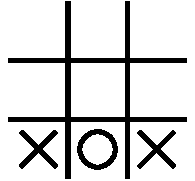
\includegraphics[scale=0.7]{04_Artefakte/01_Abbildungen/ttt_boards/ttt_163968.pdf}
   \end{minipage}%
   \begin{minipage}[c]{.5\textwidth}
      $B_G = 111000000_2$ \\
      $B_X = 101000000_2$ \\
      $B_O = 010000000_2$ \\
      $B_s = 101000000010000000_2 = 163968_{10}$
   \end{minipage}
   \caption{Beispiel für die unterschiedlichen Spielfeldkodierungen}
   \label{fig:ttt_163968}
\end{figure}

Die acht möglichen Gewinnkonstellationen $M_{i} \mid i \in [1,8]$ von \acs{TTT} können durch Bitoperationen geprüft werden.
Dafür wird eine logische AND Operation einer der Gewinnkonstellationen mit dem Bitboard eines Spielers durchgeführt und das Ergebnis auf Äquivalenz mit der ursprünglichen Gewinnkonstellation geprüft: $B_X \land M_i = M_i$. 
Ist die Äquivalenz dieser Gleichung gegeben, bedeutet dies, dass die Gewinnkonstellation $M_i$ vorliegt

Da ein Spieler nur Aktionen durchführen kann, die eine Gewinnkonstellation für ihn selbst konstruieren, muss nach einer Aktion nur das Bitboard des Spielers geprüft werden, der die letzte Aktion durchgeführt hat. 
Liegt keine Gewinnkonstellation vor und das Bitboard $B_G$ enthält keine Bits mit Wert False, endet das Spiel in einem Unentschieden.